% !Rnw weave = Sweave
\documentclass[10pt,a4paper]{report}
\usepackage{Sweave} 
\usepackage{natbib}
\usepackage{graphics}
\usepackage{amsmath}
\usepackage{indentfirst}
\usepackage{hanging}
%\usepackage{zi4}
%\usepackage[utf8]{inputenc}
\usepackage{hyperref}
\usepackage[T1]{fontenc}
\DeclareGraphicsExtensions{.png,.pdf,.jpg}

\begin{document}

%\VignetteIndexEntry{Species distribution modeling with three-step pseudo--absences}
%\VignetteDepends{mopa,sp,raster,earth}
%\VignetteKeyword{spatial}

%\newcommand{\super}[1]{\ensuremath{^{\textrm{#1}}}}
%\newcommand{\sub}[1]{\ensuremath{_{\textrm{#1}}}}
%\newcommand{\R}{{\normalfont\textsf{R }}{}}









\Sconcordance{concordance:mopa.tex:mopa.Rnw:%
1 60 1 1 2 1 0 3 1 1 4 7 0 1 2 4 1 1 3 2 0 1 1 4 0 1 2 6 1 1 2 1 0 4 1 %
3 0 1 2 2 1 1 2 4 0 1 2 3 1 1 2 1 0 1 1 1 3 6 0 1 2 6 1 1 4 3 0 2 1 4 0 %
1 2 5 1 1 4 9 0 4 1 4 0 1 2 4 1 1 5 9 0 3 1 5 0 1 3 2 1 1 5 9 0 3 1 4 0 %
1 2 2 1 1 3 5 0 1 2 6 1 1 4 6 0 1 2 12 1 1 3 8 0 1 1 1 3 6 0 1 2 2 1 1 %
2 1 0 1 1 7 0 1 2 2 1 1 2 1 0 1 5 3 0 1 1 1 2 1 0 2 1 4 0 1 2 12 1}



\title{Species distribution modeling with three-step pseudo--absences}
\author{Maialen Iturbide}
\maketitle


\chapter{Introduction}

This document provides an introduction to species distribution modeling (SDM) with three--step pseudo--absences. 

Species distribution models (SDM) are statistical tools to predict the distribution of species in geographic space based on the relation of known species distribution to the environment. SDMs can be classified into \textit{profile techniques} that only use distribution of presence data and \textit{group discrimination techniques} that also require information of the environmental range where the species do not occur, that is, absence data. Due to the great effort involved in true absences sampling, most of the available datasets for predictive modeling are lacking in absence data (\citet{zaniewski_predicting_2002}; \citet{lobo_uncertain_2010}), thereby some authors apply profile techniques such as ecological niche factor analysis (ENFA; i.e. \citet{cianfrani_habitat_2010}; \citet{mckinney_feeding_2012}), Mahalanobis distance (MADIFA: i.e. \citet{kuo_unexpected_2010}; \citet{martin_brown_2012}) and environmental envelopes (BIOCLIM and DOMAIN: i.e. \citet{giovanelli_modeling_2010}; \citet{monk_habitat_2010}). However, given that group discrimination techniques generally perform better (\citet{elith_novel_2006}; \citet{engler_improved_2004}; \citet{chefaoui_assessing_2008}), the most common  methodological approach is to use group discrimination techniques relative to the available environment or background samples, also known as pseudo--absences, thus obtaining a representation of the environmental range in the region of study. 


One of the most simple methods of generating pseudo--absences is to perform a random selection of the entire study area  (\citet{jiang_satellite-derived_2014}; \citet{maria_teresa_multi-temporal_2014}; \citet{sequeira_predicting_2014}). However, it rises the risk of introducing false absences into the model from locations that are suitable for the species. Faced with this problem, several authors employ a presence--only algorithm as a preliminary step to move pseudo--absences away in the environmental space (\citet{zaniewski_predicting_2002}; \citet{engler_improved_2004}; \citet{barbet-massin_selecting_2012}; \citet{liu_species_2013}). 

The way of generating pseudo--absences strongly influences the results obtained (\citet{lobo_uncertain_2010}; \citet{wisz_pseudo-absence_2009}; \citet{barbet-massin_selecting_2012}; \citet{hirzel_assessing_2001}), as well as the extent from which background is sampled, a constraint distribution of pseudo--absences around presence locations can lead to misleading models while the opposite, can inflate artificially test statistics and predictions, as well as potentially less informative response variables  (\citet{jeremy_vanderwal_selecting_2009}).

This document shows an example of a full Species distribution modeling process carried out with the \texttt{mopa} package in R. Pseudo--absences are generated in three-steps combining profiling techniques and background extent limitations. 

If you want to know more about SDM in R, you could consult, for example, documentation from package \texttt{dismo} made by Robert J. Hijmans and Jane Elith.


\texttt{NOTE:} Most functions presented are implemented in `mopa`. In the few cases in which functions from other packages are used, the package name is always explicitly indicated.

\chapter{Getting started}

\section{Install mopa}

The \texttt{mopa} is available on github. The `devtools` package can be used to download and install `mopa` directly from the master branch of the repository:

\begin{Schunk}
\begin{Sinput}
> if (!require(devtools)) install.packages("devtools")
> devtools::install_github("https://github.com/miturbide/mopa")
\end{Sinput}
\end{Schunk}

\begin{Schunk}
\begin{Sinput}
> library(mopa)
\end{Sinput}
\end{Schunk}

\section{Species occurrence data}

Regarding presence data, \citet{hernandez_effect_2006} suggested that research in environmental niche modeling should focus in broad distribution subunits that are based on distinct genetic linages, in this connection \citet{gonzalez_population_2011} demostrated that omission error is reduced when biologically meaningful data is modeled. Thus, functions in the \texttt{mopa} package are prepared to handle more than one group of presences at the same time (could be a list of either distribution subunits of a single species or distribution of multiple species), anyway, functions also perform with a single group or species (data frame). In this example we use a data set (list) available with the \texttt{mopa} package containing presence records of two phylogenetic groups (H11 and H5) of \textit{Quercus} sp in Europe. This is, R--object \texttt{Oak\_phylo2}, a modified subset of the \texttt{Quercus sp Europe Petit 2002} database (\citet{petit_chloroplast_2002}), which is available in the \texttt{Georeferenced Database of Genetic Diversity} or (GD)$^{2}$. To aid in map representation, a dataset called \texttt{wrld} containing a World map is also included in the package. 


\begin{Schunk}
\begin{Sinput}
> data(wrld)
> data(Oak_phylo2)
> # Map 
> plot(wrld, asp = 1, xlim= c(-10,50), ylim=c(40,60))
> for (i in 1:length(Oak_phylo2)) {
+   points(Oak_phylo2[[i]], pch = "*", cex = 0.5, 
+          col = colors()[i*50])
+ }
\end{Sinput}
\end{Schunk}
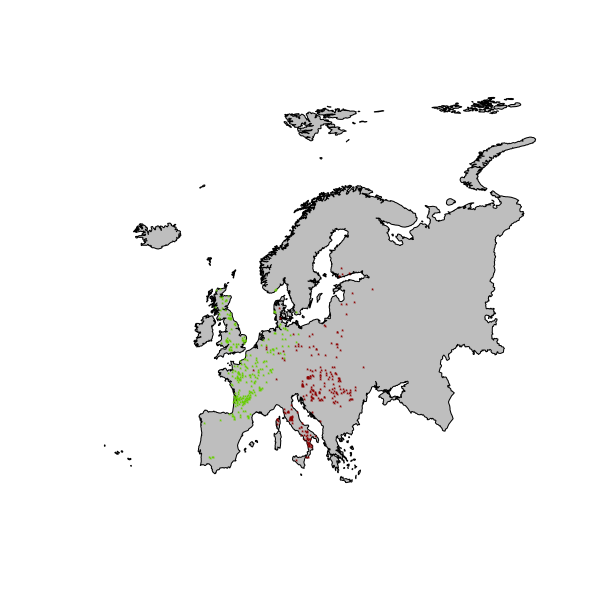
\includegraphics{mopa-mopa2}

\section{Environmental variables}

Predictor variables are typically organized as raster (grid) type files. The set of predictor variables (rasters) can be used to make a '\texttt{RasterStack}', which is a collection of '\texttt{RasterLayer}' objects (see \texttt{Raster-class} in the \texttt{raster} package for more info). \texttt{mopa} uses as input this type of raster objects and also provides the R--object \texttt{biostack}, which is a '\texttt{RasterStack}' of three bioclimatic variables.

\begin{Schunk}
\begin{Sinput}
> # RatserStack of envirinmental variables
> data(biostack)
> plot(biostack)
\end{Sinput}
\end{Schunk}
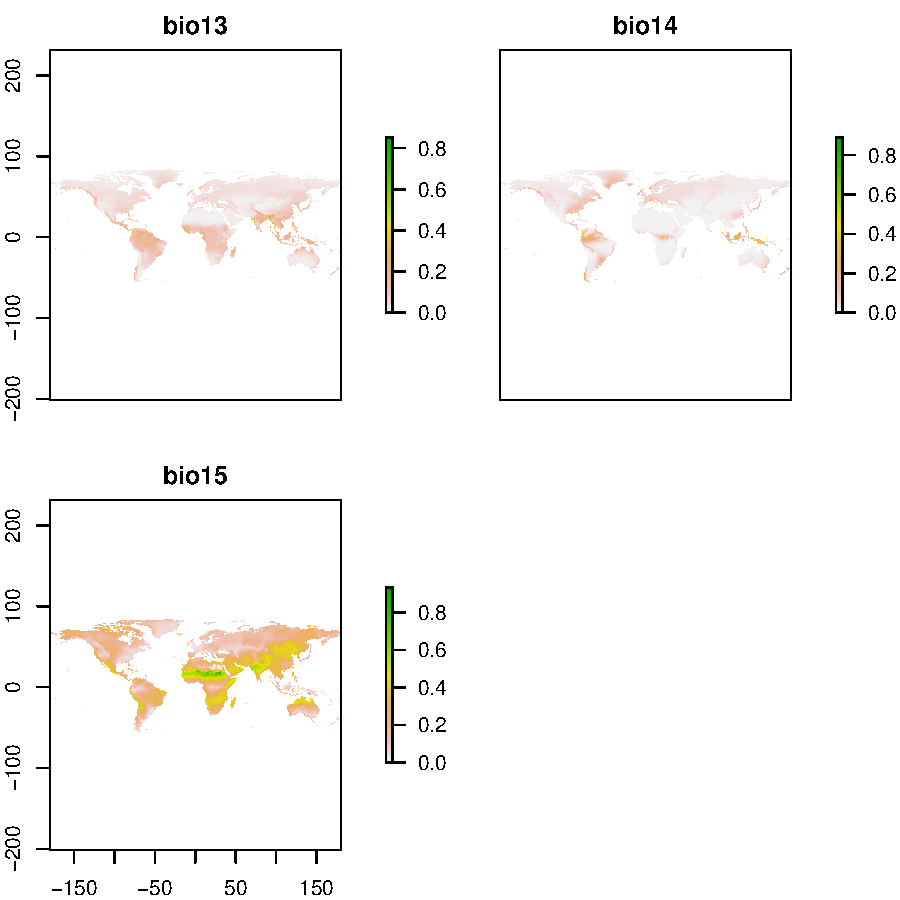
\includegraphics{mopa-mopa3}

\chapter{Study area and background}

\section{Creation of the background grid}

The regular point grid which covers the continental area can be created with functions from the \texttt{raster} and \texttt{sp} packages as follows:

\begin{Schunk}
\begin{Sinput}
> library(raster)
> ac<-xyFromCell(biostack[[1]],  1:ncell(biostack[[1]]))
> ex<-extract(biostack[[1]], ac)
> sp_grid<-SpatialPoints(ac[-which(is.na(ex)),])
> projection(sp_grid)<-CRS("+proj=longlat +init=epsg:4326")
\end{Sinput}
\end{Schunk}

For easy of use, R--object \texttt{sp\_grid} is available in \texttt{mopa}, covering the World at 10 km resolution.

\section{Limit study area to the bounding boxes around presences}

Function \texttt{boundingCoords} creates the matrix of bounding coordinates around point records (xy records). In this case, since \texttt{Oak\_phylo2} object is a list of two groups of points, a list of two matrixes is created.

\begin{Schunk}
\begin{Sinput}
>  oak.extension <- boundingCoords(xy = Oak_phylo2)
\end{Sinput}
\end{Schunk}

Function \texttt{delimit} creates polygon shapes from bounding coordinates and limits \texttt{SpatialPoints} data (\texttt{sp\_grid}) to the defined boundaries, in other words, does the intersection of the background point grid with the bounding boxes. A list with two objects is obtained, (1)bbs: polygon shape of the bounding boxes and (2)bbs.grid: list of data frames of the background point grid limited by the bounding boxes.


\begin{Schunk}
\begin{Sinput}
> box.grid <- delimit(bounding.coords = oak.extension, 
+               grid = sp_grid, names = names(Oak_phylo2))
> # Plot presences and bounding boxes
> plot(box.grid$bbs, asp = 1)
> for (i in 1:length(Oak_phylo2)){
+   points(Oak_phylo2[[i]], col = colors()[i*50])
+ }
\end{Sinput}
\end{Schunk}
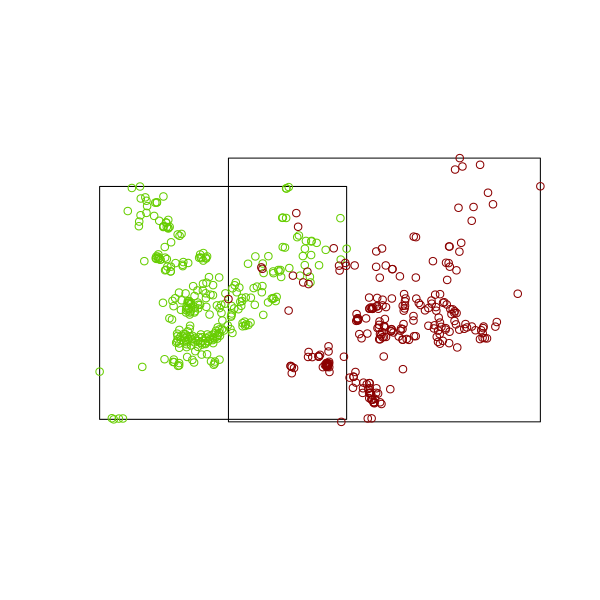
\includegraphics{mopa-mopa6}


\chapter{Three--step pseudo--absences generation}

In this chapter we illustrate the steps to generate pseudo-absences in three-steps combining profiling techniques and background extent limitations. 

\section{STEP1: environmental profiling}

The first step is the selection of the environmentally unsuitable areas with a presence only algorithm. function \texttt{OCSVMprofiling} uses One-class support vector machines (OCSVM) (\citet{scholkopf_learning_2001}) to perform a preliminary binary classification of the study region (suitable/unsuitable) using as input the environmental conditions of the presence localities.

\begin{Schunk}
\begin{Sinput}
> unsuitable.bg <-OCSVMprofiling(xy = Oak_phylo2, 
+                     varstack = biostack, 
+                     bbs.grid = box.grid$bbs.grid)
> # Plot areas predicted as suitable (presence) and 
> # unsuitable (absence) for group H11
> plot(unsuitable.bg$absence$H11, pch = "*", asp = 1)
> points(unsuitable.bg$presence$H11, pch = "*", col = "pink2")
\end{Sinput}
\end{Schunk}
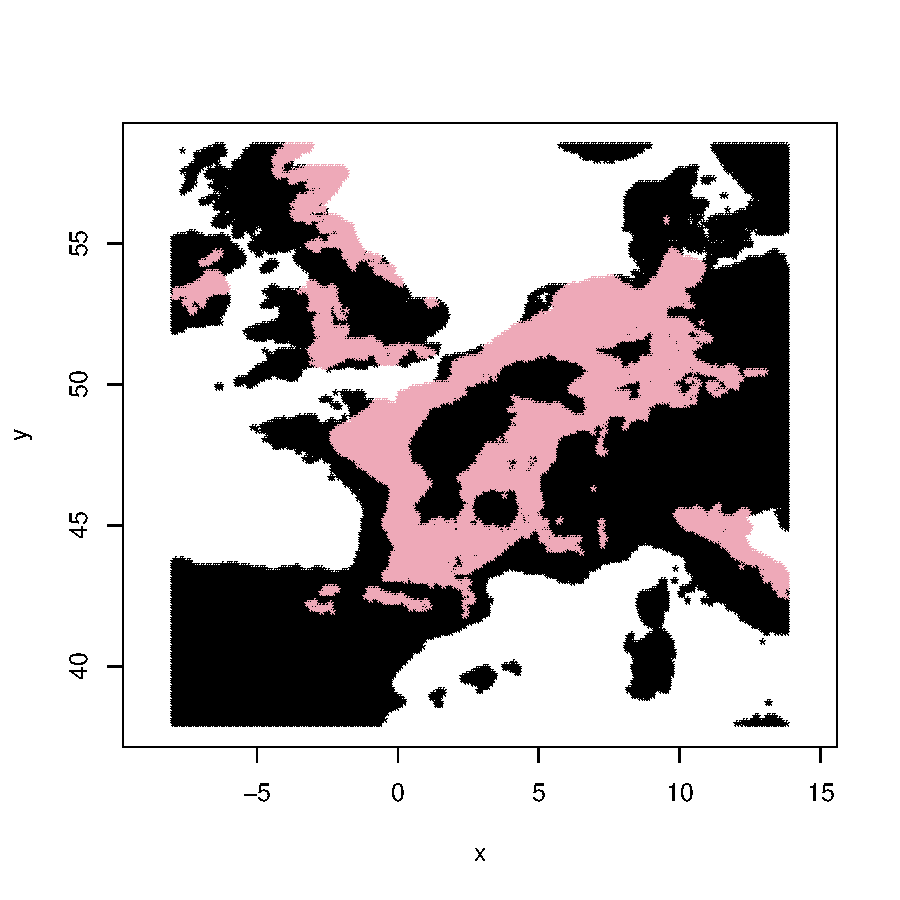
\includegraphics{mopa-mopa7}


\section{STEP2: SDM performing with pseudo--absences generated into different extents of the unsuitable background}

In the second step, SDMs are performed with pseudo--absences generated into different extents of the unsuitable background. Several functions are involved in this step. Function \texttt{bgRadio} performs the partition of the background space considering multiple distance thresholds. In other words, it creates backgrounds of different spatial extent for each species/population. In the example below, extents are created for a sequence of 10 km between distances, from 20 km to half the length of the diagonal of the bounding box, as described in Sec. 2.4 of the manuscript. A list of matrices containing xy coordinates is returned, each matrix corresponding to a different background extent tested.

\begin{Schunk}
\begin{Sinput}
> ext <- bgRadio(xy = Oak_phylo2, bounding.coords = oak.extension, 
+                bg.absence = unsuitable.bg$absence, 
+                start = 0.166, by = 0.083, 
+                unit = "decimal degrees")
\end{Sinput}
\begin{Soutput}
[1] "creating background point-grids for species 1 out of 2"
[1] "creating background point-grids for species 2 out of 2"
\end{Soutput}
\begin{Sinput}
> # Plot presences for group H11 and background extents of 20, 
> # 120 and 520 km
> plot(ext$H11$km520, col = "green4", pch = "*", asp = 1)
> points(ext$H11$km120, pch = "*")
> points(ext$H11$km20, pch = "*", col = "blue")
> points(Oak_phylo2$H11, col = "red", pch = ".", cex = 1.5)
\end{Sinput}
\end{Schunk}
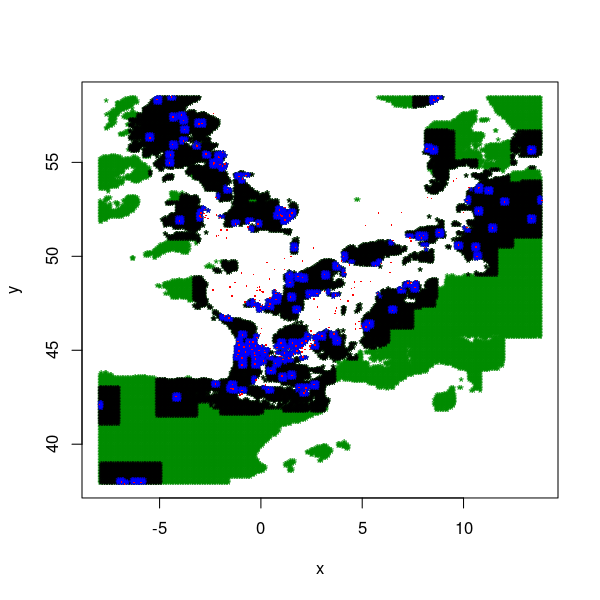
\includegraphics{mopa-mopa8}

With function \texttt{PseudoAbsences}, you can create pseudo--absences either at random or with k--means clustering, by modifying argument \texttt{kmeans}. You can also set the prevalence (proportion of presences against pseudo--absences) and the exclusion buffer (minimum distance to be kept to presences without pseudo--absences).

\subsection{At random}

In the example below, pseudo--absences are generated at random, in equal number to presences (prevalence) and keeping a 10 km distance to presences (exclusion buffer).



\begin{Schunk}
\begin{Sinput}
> pa_random <-PseudoAbsences(xy = Oak_phylo2, bg.grids = ext, 
+                            exclusion.buffer = 0.083, 
+                            prevalence = 0.5, kmeans = FALSE)
\end{Sinput}
\begin{Soutput}
[1] "generating pseudo-absences for species 1 out of 2"
[1] "generating pseudo-absences for species 2 out of 2"
\end{Soutput}
\begin{Sinput}
> # Plot presences/pseudo-absences for group H11 considering 
> # the background extent of 520 km
> plot(ext$H11$km520, pch="*", col= "grey", cex=.5, asp=1)
> points(pa_random$H11$km520, col= "red", pch=".", cex=4)
> points(Oak_phylo2$H11, col= "blue", pch=".", cex=3)
\end{Sinput}
\end{Schunk}
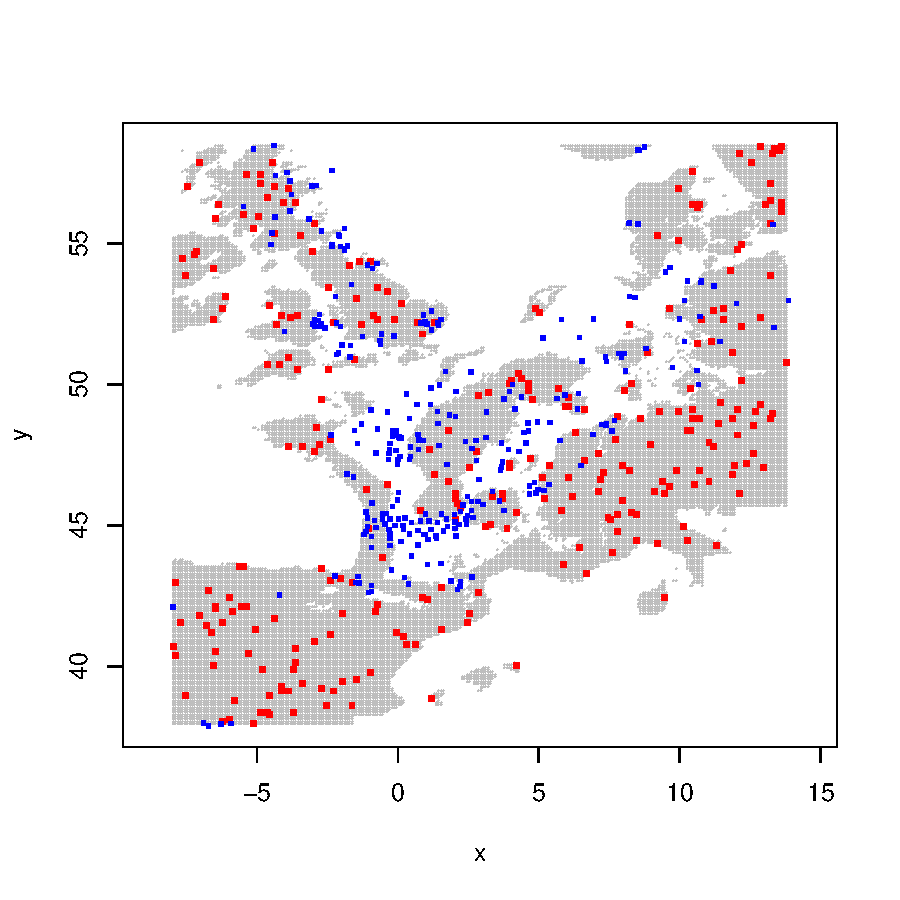
\includegraphics{mopa-mopa9}

\subsection{With k--means clustering}

In the example below, pseudo-absences are generated with k-means clustering, in equal number to presences (prevalence) and keeping a 10 km distance to presences (exclusion buffer).

\begin{Schunk}
\begin{Sinput}
> pa_kmeans <-PseudoAbsences(xy = Oak_phylo2, bg.grids = ext, 
+                            exclusion.buffer = 0.083, 
+                            prevalence = 0.5, kmeans = TRUE, 
+                            varstack = biostack)
\end{Sinput}
\begin{Soutput}
[1] "generating pseudo-absences for species 1 out of 2"
[1] "generating pseudo-absences for species 2 out of 2"
\end{Soutput}
\begin{Sinput}
> # Plot presences/pseudo-absences for group H11 considering 
> # the background extent of 520 km
> plot(ext$H11$km520, pch = "*", col = "grey", cex = .5, asp = 1)
> points(pa_kmeans$H11$km520, col = "red", pch = ".", cex = 4)
> points(Oak_phylo2$H11, col = "blue", pch = ".", cex = 3)
\end{Sinput}
\end{Schunk}
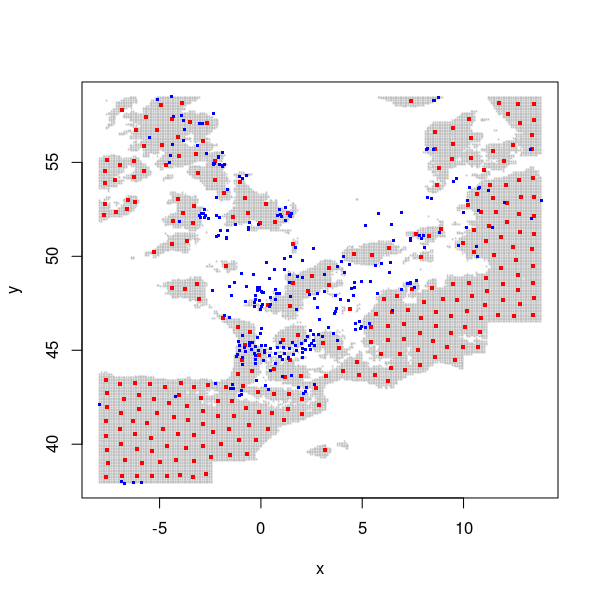
\includegraphics{mopa-mopa10}


Function \texttt{bindPresAbs} binds presence and absence data for each background extension.

\begin{Schunk}
\begin{Sinput}
> presaus <- bindPresAbs(presences = Oak_phylo2, 
+                        absences = pa_random)
\end{Sinput}
\end{Schunk}


The \texttt{allModeling} function does the species distribution modelling and k-fold cross validation for a set of presence/absence data per species corresponding to a different background 
extent. Algorithms supported are "glm", "svm", "maxent", "mars", "randomForest", "cart.rpart" 
and "cart.tree".

In the example below, we do a 10--fold cross validation of the "mars" modelling algorithm.

\begin{Schunk}
\begin{Sinput}
> modirs <- allModeling(data = presaus, varstack = biostack, 
+             k = 10, algorithm = "mars", destdir = getwd(), 
+             projection = CRS("+proj=longlat +init=epsg:4326"))
\end{Sinput}
\end{Schunk}

Named Rdata objects are stored in the specified path. Each Object is given a name indicating the algorithm, background extent, and species in this order (if a single species is provided no name is given for de species). Character object with listed files is returned. Each Rdata consists of a list with six components:

	(1)allmod: fitted model with all data for training, 
	(2)auc: AUC statistic in the cross validation,
	(3)kappa: kappa statistic in the cross validation,
	(4)tss: true skill statistic in the cross validation,
	(5)mod: fitted model with partitioned data, 
	(6)p: cross model prediction. 

\section{STEP3: selection of the optimum background extent and corresponding fitted model}

In the third step, AUCs obtained and corresponding extents are fitted to a Michaelis-Menten model to extract the \textit{Vm} coefficient (equation 1 in the manuscript). Then, the minimum extent at which the AUC surpasses the \textit{Vm} value is selected as the threshold extent (see Figure 3 in the manuscript), being the corresponding fitted SDM the definitive to predict suitability probabilities in the study area.

We next indicate how to plot the results of the optimal spatial extent selection using the `lattice` package. First we load the data generated with the  \texttt{allModeling} function and extract the corresponding AUC values. Function  \texttt{loadTestValues} loads and stores AUC data in a matrix:

\begin{Schunk}
\begin{Sinput}
> auc_mars <-loadTestValues(data = presaus, test = "auc", 
+                           algorithm = "mars")
\end{Sinput}
\begin{Soutput}
[1] "loading values for species 1"
[1] "loading values for species 2"
\end{Soutput}
\end{Schunk}
\includegraphics{mopa-mopa13}


Model fitting is done by function \texttt{indextent}, that internally uses the  \texttt{nls} function of R package  \texttt{stats}. An index of the threshold extents is obtained. A fitted model plot is also returned if argument  \texttt{diagrams} is set to  \texttt{TRUE} (the point crossed by the vertical line above the horizontal line corresponds to the smallest background extent at which the AUC overcomes the `Vm` value (threshold extent)).

\begin{Schunk}
\begin{Sinput}
> ind <- indextent(testmat = auc_mars, diagrams = TRUE)
> ind
\end{Sinput}
\begin{Soutput}
km370 km230 
   36    22 
\end{Soutput}
\end{Schunk}
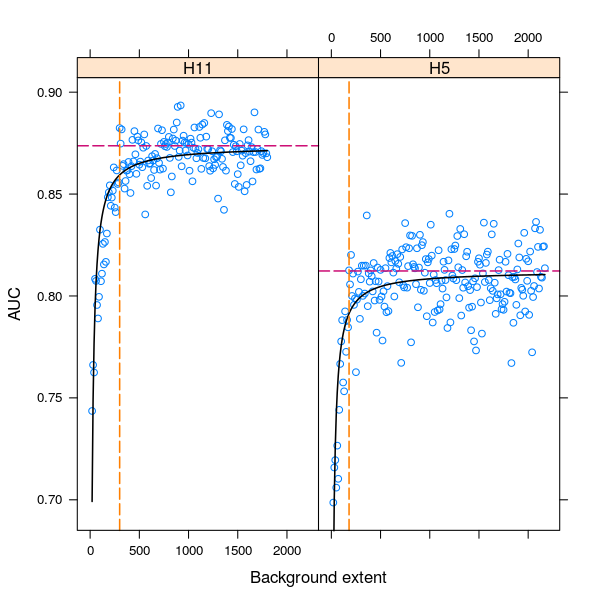
\includegraphics{mopa-mopa14}

Thus, the \texttt{ind} object in this example gives the index of the background extents to be considered for each group/species and is used to extract definitive model components and data with function \texttt{loadDefinitiveModel} as follows. 

\begin{Schunk}
\begin{Sinput}
> def <-loadDefinitiveModel(data = presaus, extents = ind, 
+                      slot = "allmod", algorithm = "mars")
\end{Sinput}
\end{Schunk}

Once the optimal SDMs are chosen, we can generate the resulting suitability maps. In the example below we use function \texttt{biomat} for preparing a matrix with the variables for prediction in the study area. Then, the predictions are converted to a raster format with functions \texttt{SpatialPixelsDataFrame} (from the \texttt{sp} package) and \texttt{raster} (from the \texttt{raster} package).

\begin{Schunk}
\begin{Sinput}
> # Suitability map for the Oak group H11
> # Function 'biomat' prepares matrix with variables for 
> # projection
> projectionland <- biomat(cbind(box.grid$bbs.grid$H11, 
+                         rep(1, nrow(box.grid$bbs.grid$H11))), 
+                         biostack)
> # Prediction
> p <- predict(def$H11, projectionland[ ,-1])
> p[which(p < 0)] <- 0
> p[which(p > 1)] <- 1
> # Convert prediction to a raster object
> spp <- SpatialPixelsDataFrame(box.grid$bbs.grid$H11, 
+                               as.data.frame(p))
> ras <- raster(spp)
> plot(ras)
\end{Sinput}
\end{Schunk}
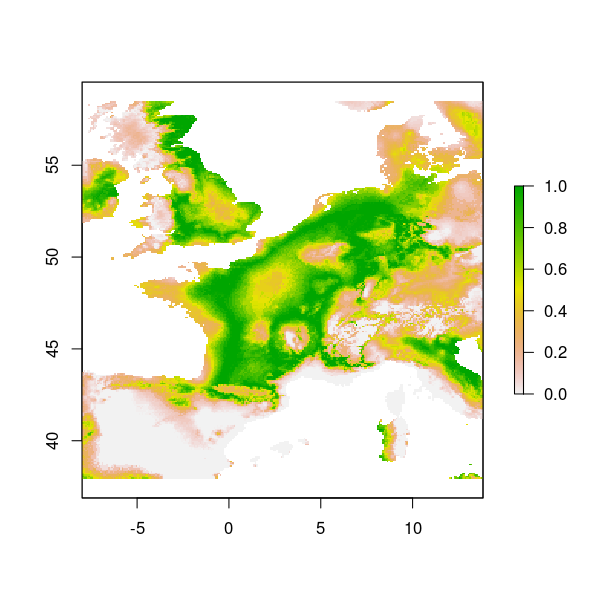
\includegraphics{mopa-mopa16}



%unsrtnat
\bibliographystyle{elsarticle-harv}
\bibliography{gen2}



\end{document}


